\newpage
%\thispagestyle{empty}
%Modifique a estrutura dos capítulos e seções de acordo com a necessidade do seu trabalho
\section{METODOLOGIA}
Toda a execução do projeto será realizada por microcomputador presente no parque computacional da instituição. Serão utilizadas as linguagens HTML, PHP, Java e JavaScript e o software Weka, que já se mostraram ser uma boa escolha em desenvolvimento de softwares esportivos scout. 
 
A construção do software será modularizada, conforme podemos observar na figura 1. A montagem da base de dados será baseada nas bases de dados existentes na literatura e deverá ser capaz de armazenar diferentes modelagens em uma única base. O primeiro módulo, selecionar, é o responsável por selecionar: a base de dados e partida desejada. O próximo módulo, visualizar, é o responsável por apresentar os dados do jogo através dos seus quatro elementos do processo de scout: espaço (imagens de campo), tempo (escolha do tempo da partida), jogador(escalação) e fundamento (tabelas de dados). Já o terceiro e o quarto módulo, otimizar e relatório permite ao usuário projetar e visualizar os relatórios com a compilação das informações proveniente da base de dados.

\begin{figure}[htbp]
  \begin{center}
  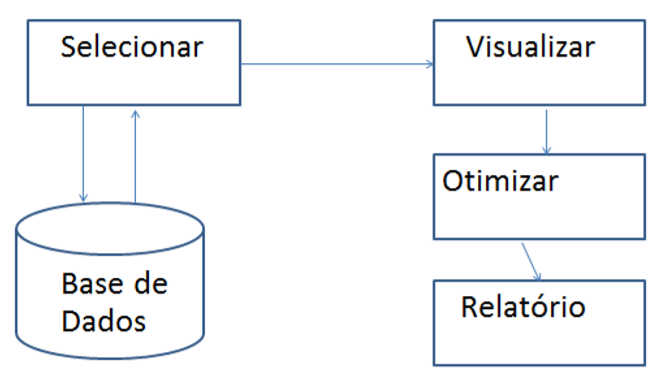
\includegraphics[width=.5\linewidth]{imagens/fluxograma.png}\\
  \end{center}
  \caption[Fluxograma do sistema proposto]{Fluxograma do sistema proposto}
  \label{fig:logo}
  %\legend{Fonte: Próprio Autor}
\end{figure}